\documentclass[12pt,english,a4paper]{report}
\pdfobjcompresslevel=0
\usepackage[usenames,dvipsnames]{xcolor}
\usepackage[includeheadfoot,margin=0.8 in,top=0.6 in]{geometry}
\usepackage{siunitx,physics,cancel,upgreek,varioref,listings,booktabs,tocloft, pdfpages}
\usepackage{mathtools}
\usepackage{babel}
\usepackage{graphicx}
\usepackage{float}
\usepackage{fouriernc}
\usepackage{fancyhdr}
\usepackage[utf8]{inputenc}
\usepackage{amsmath}
\usepackage{amssymb}
\usepackage{textcomp}
\usepackage{lastpage}
\usepackage{microtype}
\usepackage[linktoc=all, bookmarks=true, pdfauthor={Anders Johansson}]{hyperref}
\renewcommand{\CancelColor}{\color{red}}
\renewcommand{\exp}[1]{\mathrm{e}^{#1}}
\newcommand{\R}{\mathbb{R}}
\newcommand{\tittel}[1]{\title{#1 \vspace{-7ex}}\author{}\date{}\maketitle\thispagestyle{fancy}\pagestyle{fancy}\setcounter{page}{1}}

\newcommand{\deloppg}[2][]{\subsection*{#2) #1}\addcontentsline{toc}{subsection}{#2)}\refstepcounter{subsection}\label{#2}}
\newcommand{\oppg}[1]{\section*{Oppgave #1}\addcontentsline{toc}{section}{Oppgave #1}\refstepcounter{section}\label{oppg#1}}

\labelformat{section}{section~#1}
\labelformat{subsection}{section~#1}
\labelformat{subsubsection}{paragraph~#1}
\labelformat{equation}{equation~(#1)}
\labelformat{figure}{figure~#1}
\labelformat{table}{table~#1}

\lstset{rangeprefix=/*\#,
rangesuffix=\#*/,
includerangemarker=false}
\renewcommand{\lstlistingname}{Code snippet}
\definecolor{codegreen}{rgb}{0,0.6,0}
\definecolor{codegray}{rgb}{0.5,0.5,0.5}
\definecolor{codepurple}{rgb}{0.58,0,0.82}
\definecolor{backcolour}{rgb}{0.95,0.95,0.92}
\lstset{showstringspaces=false,
basicstyle=\footnotesize\ttfamily,
keywordstyle=\color{codegreen},
commentstyle=\color{magenta},
numberstyle=\tiny\color{codegray},
stringstyle=\color{codepurple},
frameshape={RYRYNYYYY}{yny}{yny}{RYRYNYYYY},
breaklines=true,
literate={0}{{\textcolor{blue}{0}}}{1}%
             {1}{{\textcolor{blue}{1}}}{1}%
             {2}{{\textcolor{blue}{2}}}{1}%
             {3}{{\textcolor{blue}{3}}}{1}%
             {4}{{\textcolor{blue}{4}}}{1}%
             {5}{{\textcolor{blue}{5}}}{1}%
             {6}{{\textcolor{blue}{6}}}{1}%
             {7}{{\textcolor{blue}{7}}}{1}%
             {8}{{\textcolor{blue}{8}}}{1}%
             {9}{{\textcolor{blue}{9}}}{1}%
             {.0}{{\textcolor{blue}{.0}}}{2}% Following is to ensure that only periods
             {.1}{{\textcolor{blue}{.1}}}{2}% followed by a digit are changed.
             {.2}{{\textcolor{blue}{.2}}}{2}%
             {.3}{{\textcolor{blue}{.3}}}{2}%
             {.4}{{\textcolor{blue}{.4}}}{2}%
             {.5}{{\textcolor{blue}{.5}}}{2}%
             {.6}{{\textcolor{blue}{.6}}}{2}%
             {.7}{{\textcolor{blue}{.7}}}{2}%
             {.8}{{\textcolor{blue}{.8}}}{2}%
             {.9}{{\textcolor{blue}{.9}}}{2}%
}

\renewcommand{\footrulewidth}{\headrulewidth}
\tocloftpagestyle{fancy}

\setcounter{secnumdepth}{4}
\renewcommand{\thesection}{\arabic{section}}
\renewcommand{\thesubsection}{\arabic{section}.\arabic{subsection}}
\renewcommand{\thesubsubsection}{\arabic{section}.\arabic{subsection}.\arabic{subsubsection}}
\setlength{\parindent}{0cm}
\setlength{\parskip}{1em}

\newcommand{\eqtag}[1]{\refstepcounter{equation}\tag{\theequation}\label{#1}}
\hypersetup{colorlinks=true,urlcolor=blue,linkcolor=black}

\sisetup{detect-all}
\sisetup{exponent-product = \cdot, output-product = \cdot,per-mode=symbol}
\sisetup{output-decimal-marker={.}}
\sisetup{round-mode = off, round-precision=3}
\sisetup{number-unit-product = \ }
\DeclareSIUnit\year{yr}

\allowdisplaybreaks[4]
\fancyhf{}

\rhead{Anders Johansson}
\rfoot{Page \thepage{} of \pageref{LastPage}}
\lhead{FYS3150}
%
\usepackage[backend=biber,citestyle=numeric-comp,bibstyle=numeric,sorting=none]{biblatex}
\DefineBibliographyStrings{norsk}{%
  bibliography = {Referanser},
}
\DefineBibliographyStrings{english}{%
  bibliography = {References},
}
\addbibresource{kilder.bib}

\begin{document}
%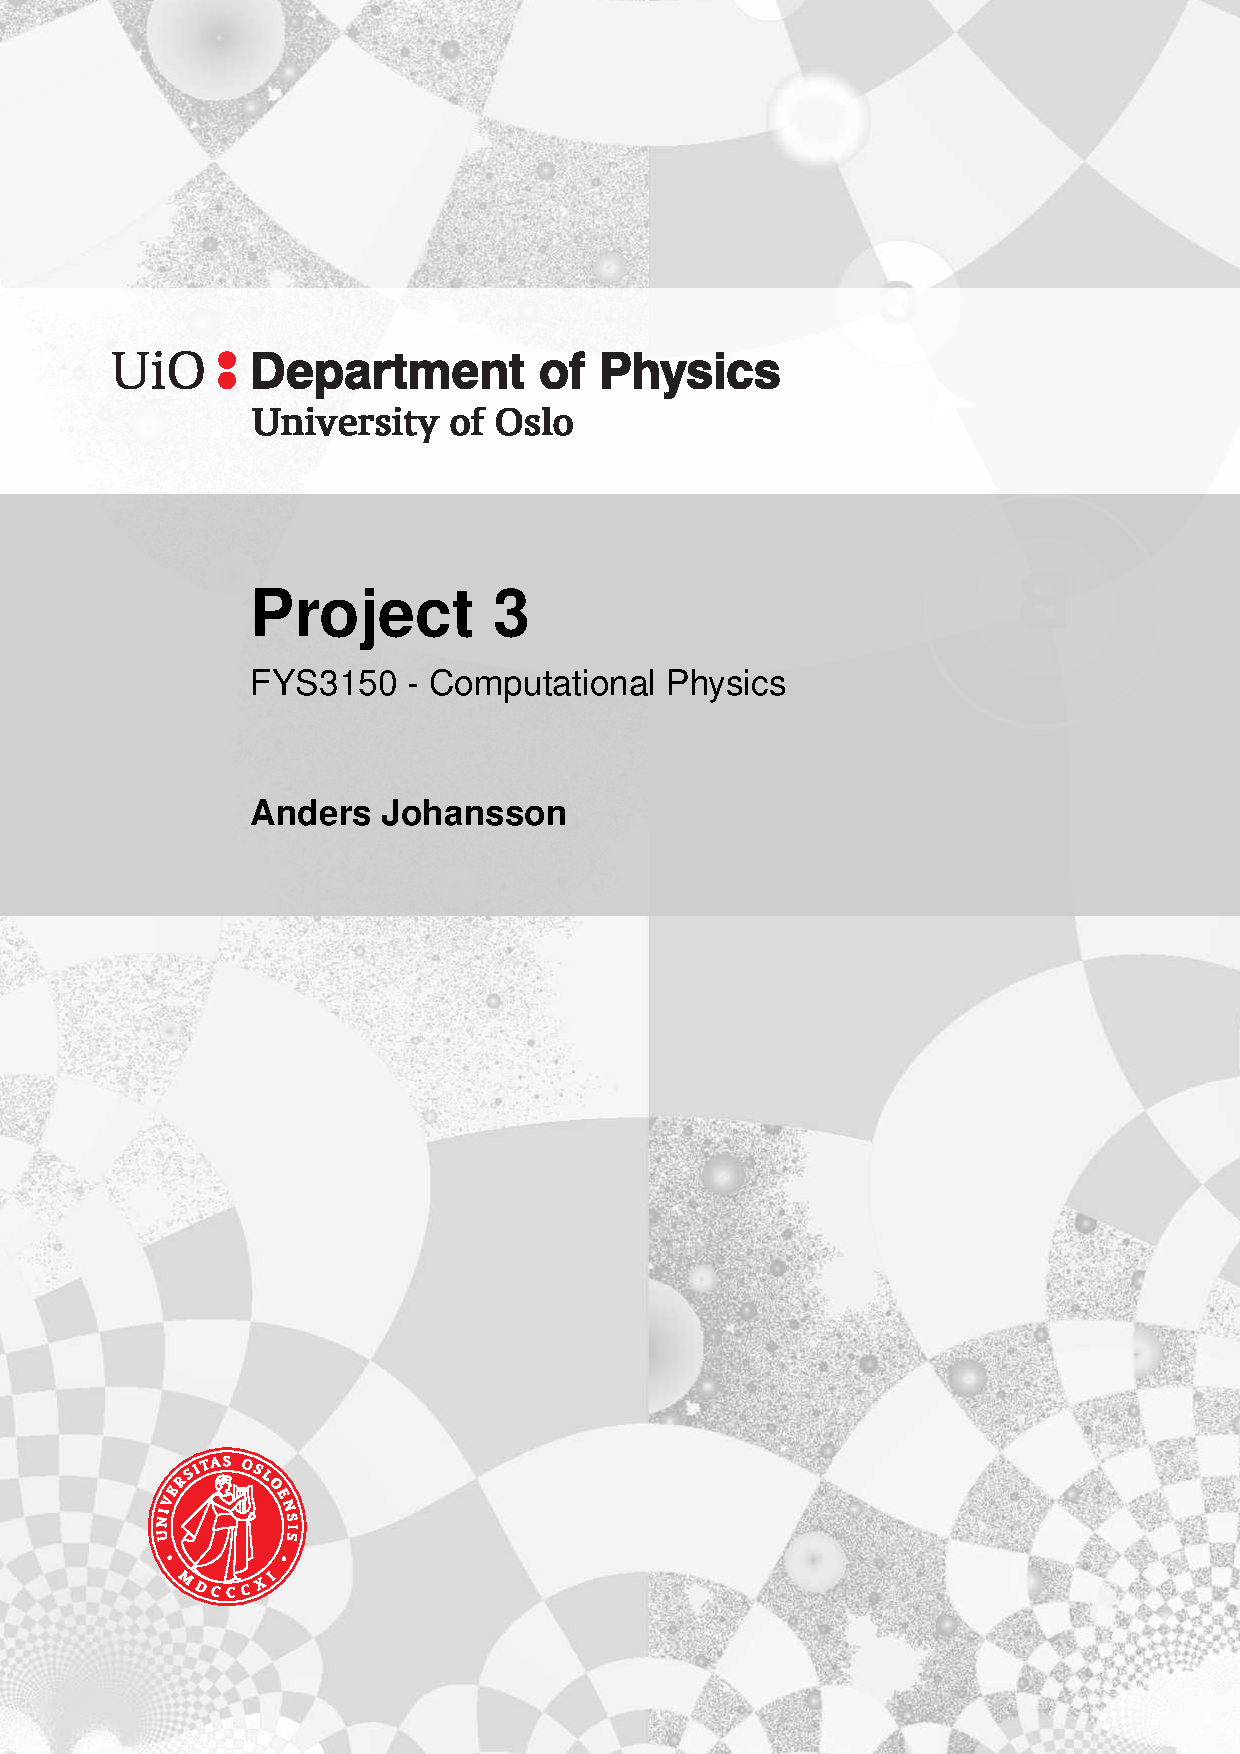
\includepdf{forside.pdf}
\pagestyle{fancy}
\tableofcontents

%      _             _
%  ___| |_ __ _ _ __| |_
% / __| __/ _` | '__| __|
% \__ \ || (_| | |  | |_
% |___/\__\__,_|_|   \__|
%

\section{Abstract}
\section{Introduction}


%   __           _ _    _
%  / _|_   _ ___(_) | _| | __
% | |_| | | / __| | |/ / |/ /
% |  _| |_| \__ \ |   <|   <
% |_|  \__, |___/_|_|\_\_|\_\
%      |___/

\section{Physical theory}
\subsection{Gravitation}
In this project, a solar system will be studied. By solar system, I mean a system where only gravitational forces effect the bodies, and where there is a large mass fixed in origo\footnote{This is a reasonable approximation, as the mass of the sun is much larger than the masses of the planets.}. Newtons gravitational law states that the gravitational force on a body with mass \(m\) from another body with mass \(M\) and relative position \(\vec{r}\) is given by
\[
\vec{F}_\mathrm{G} = -\frac{GmM}{\norm{\vec{r}}^2}\vec{r}
\]
where \(G\) is the gravitational constant, \(\SI{6.67e-11}{\N\meter\squared\per\second\squared}\). The direction of the force is given by the fact that gravity is an attractive force. If one of the objects is the sun, the mass is denoted by \(M_\odot\). With the sun placed in origo, \(r\) is simply the norm of the position vector of the planet with mass \(m\).

If there are \(n\) planets in the solar system, in addition to the sun, the sum of the forces on planet \(i\) with mass \(m_i\) is
\begin{alignat*}{2}
\sum{\vec{F}_i} &= \sum_{\substack{j=0\\j\neq i}}^n\frac{Gm_im_j}{\norm{\vec{r}_i-\vec{r}_j}^3}\qty(\vec{r}_i-\vec{r}_j)
\intertext{with \(m_0=M_\odot\) and \(\vec{r}_0=\vec{0}\). From Newton's second law, we know that \(\sum{\vec{F}_i}=m_i\vec{a}_i\), so the acceleration of planet \(i\) is given by}
\vec{a}_i &= \sum_{\substack{j=0\\j\neq i}}^n \frac{Gm_j}{\norm{\vec{r}_i-\vec{r}_j}^3}\qty(\vec{r}_i-\vec{r}_j) \eqtag{avec}
\end{alignat*}
As the sun has been fixed to origo, \(\vec{a}_0\) is set to \(\vec{0}\).


%             _          _
%   ___ _ __ | |__   ___| |_ ___ _ __
%  / _ \ '_ \| '_ \ / _ \ __/ _ \ '__|
% |  __/ | | | | | |  __/ ||  __/ |
%  \___|_| |_|_| |_|\___|\__\___|_|
%


\subsection{Choice of units}
In the solar system, seconds and meters are unpractical, as planets are millions of kilometers apart and take years to do one lap around the sun. As such, it is common to use so-called astronomical units, where \(\SI{1}{\astronomicalunit}\) is the mean distance between the sun and the earth, and time is measured in years. To express the gravitational constant in these units, we can use that if the earth were moving in a circle around the sun, the acceleration in Newton's second law would be given by the sentripetal acceleration:
\[
\frac{mv^2}{r} = \frac{GmM_\odot}{r^2} \implies G = \frac{rv^2}{M_\odot} = \SI{1}{\astronomicalunit}\cdot\qty(\frac{2\pi\cdot\SI{1}{\astronomicalunit}}{M_\odot\cdot\SI{1}{\year}})^2 = \frac{4\pi^2}{M_\odot}\  \si{\astronomicalunit\tothe3\per\year\squared}
\]
With this change of units, \vref{avec} can be written as
\[
\vec{a}_i = \sum_{\substack{j=0\\j\neq i}}^n 4\pi^2\frac{m_j}{M_\odot}\frac{\vec{r}_i-\vec{r}_j}{\norm{\vec{r}_i-\vec{r}_j}^3}\cdot \SI{1}{\astronomicalunit\cubed\per\year\squared} \eqtag{avecast}
\]


%                  _                       _   _ _    _
%  _ __ ___   __ _| |_ ___ _ __ ___   __ _| |_(_) | _| | __
% | '_ ` _ \ / _` | __/ _ \ '_ ` _ \ / _` | __| | |/ / |/ /
% | | | | | | (_| | ||  __/ | | | | | (_| | |_| |   <|   <
% |_| |_| |_|\__,_|\__\___|_| |_| |_|\__,_|\__|_|_|\_\_|\_\
%

\section{Mathematical theory}









\clearpage
\addcontentsline{toc}{section}{References}
\printbibliography


\end{document}
